\documentclass{article}
\usepackage[utf8]{inputenc}
\usepackage[margin = 0.8in]{geometry}
\usepackage{graphicx}
\usepackage{amsmath, amssymb}
\usepackage{subcaption}
\usepackage{multirow}
\usepackage{mathtools}
\usepackage{float}


\title{RBE549 - Homework 4}
\author{Keith Chester}
\date{Due date: September 29, 2022}

\begin{document}
\maketitle

\section*{Problem 0}

I am going to be working with Bob DeMont and Zeke Flaton for the final project. We will be utilizing CARLA, a self driving car simulator, to demonstrate a real world application of semantic or instance segmentation. Additional details will come with the project proposal.


\section*{Problem 1}

In this problem we are tasked with using OpenCV to compute and display the Hough lines on a given image. All code to generate these outputs can be found in $problem1.py$.

First we grab our chosen artwork.

\begin{figure}[H]
    \centering
    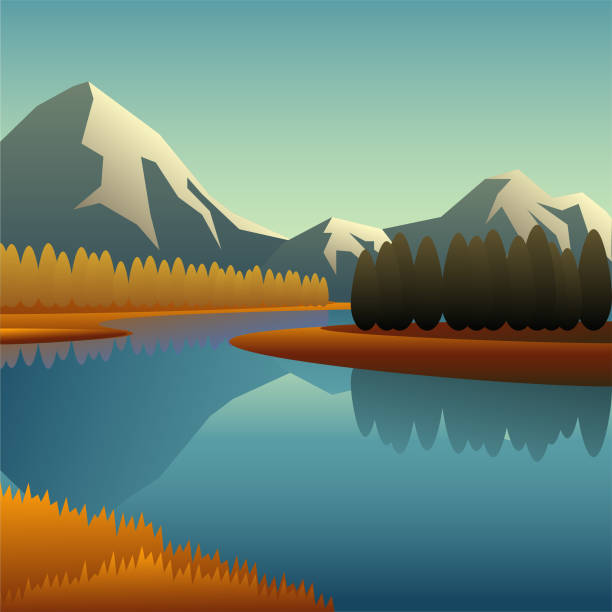
\includegraphics[width = 0.45\textwidth]{imgs/original.jpg}
    \caption{Original image}
    \label{fig:1-1}
\end{figure}

From here, we graysale the image and then apply a Gaussian blur as that's known to improve edge detection. We then try to get a Sobel edge detection.

\begin{figure}[H]
    \centering
    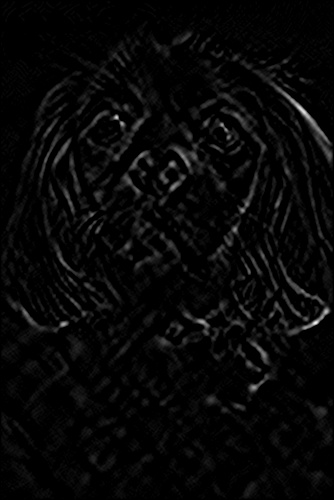
\includegraphics[width = 0.45\textwidth]{imgs/sobel.jpg}
    \caption{Sobel of images}
    \label{fig:1-2}
\end{figure}

We then find and display the Hough Lines of this image. This does not, however, work out great.

\begin{figure}[H]
    \centering
    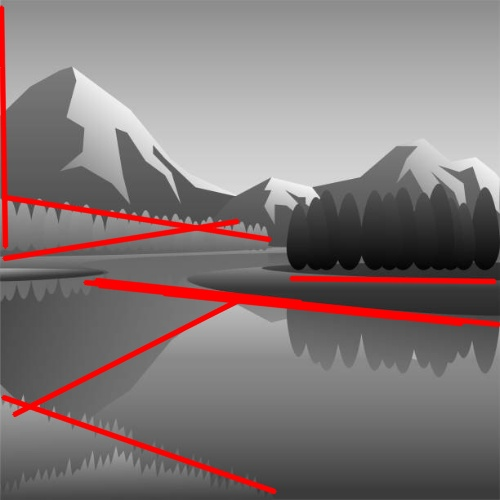
\includegraphics[width = 0.45\textwidth]{imgs/hough_lines_sobel.jpg}
    \caption{Sobel + Hough Lines}
    \label{fig:1-3}
\end{figure}

To get better results, we swap to Canny edge detection:

\begin{figure}[H]
    \centering
    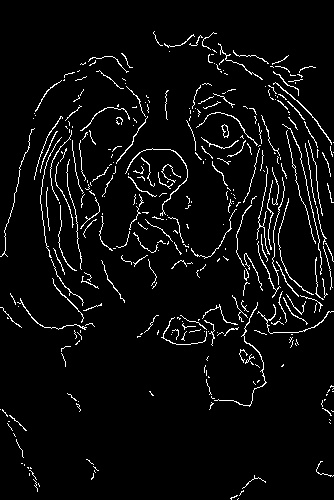
\includegraphics[width = 0.45\textwidth]{imgs/canny.jpg}
    \caption{Canny Edges}
    \label{fig:1-4}
\end{figure}

This results in a better outcome, with edges clearly delineated.

\begin{figure}[H]
    \centering
    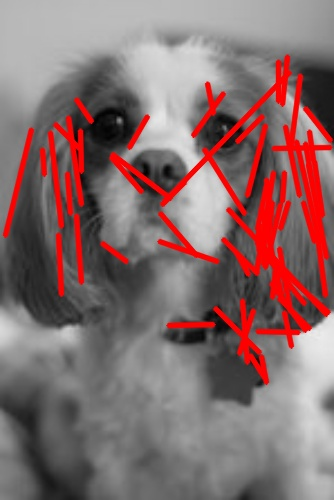
\includegraphics[width = 0.45\textwidth]{imgs/hough_lines_canny.jpg}
    \caption{Canny + Hough Lines}
    \label{fig:1-5}
\end{figure}

We can then isolate the peak Hough line by isolating the strongest line, seen here:

\begin{figure}[H]
    \centering
    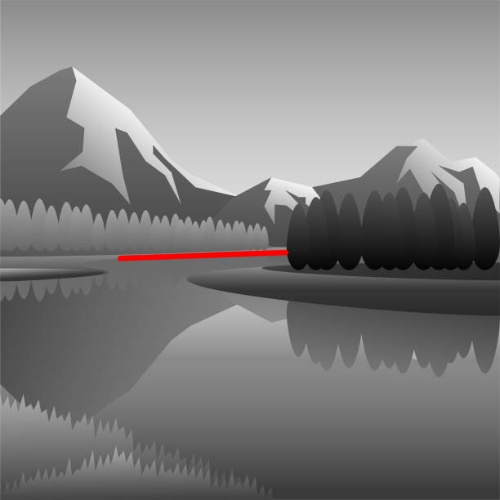
\includegraphics[width = 0.45\textwidth]{imgs/hough_lines_peak_line.jpg}
    \caption{Peak Hough Line}
    \label{fig:1-6}
\end{figure}


\section*{Problem 2}

In this problem, we are looking at a Hough Transform problem where $x$, $y$, $b$, $c$, $m$, and $n$ may be positive or negative real numbers. $2$ points in $(x,y)$ space are given by $P_1=(2,4)$ and $P_2=(4,3)$.

\subsection*{A}

First, we are tasked with finding $L_1$ and $L_2$, the lines assoicated in $(m,b)$ space corresponding to $P_1$ and $P_2$.

For this we must first solve for $m$ and $b$ to form lines for $(m,b)$ space. Given that $y = mx + b$, we have:

\begin{equation}
    L_1: 4 = 2m + b
\end{equation}

\begin{equation}
    L_1: b = -2m + 4
\end{equation}

\begin{equation}
    L_2: 3 = 4m + b
\end{equation}

\begin{equation}
    L_2: b = -4m + 3
\end{equation}

\subsection*{B}

Next we are tasked with finding the intersection of these lines. Thus we can set $L_1=L_2$ and find:

\begin{equation}
    -2m + 4 = -4m + 3
\end{equation}

\begin{equation}
    1 = -2m
\end{equation}

\begin{equation}
    m = -\frac{1}{2}
\end{equation}

\noindent ...and then solve for $b$ using our discovered $m$:

\begin{equation}
    b = -2(-\frac{1}{2}) + 4 = 5
\end{equation}

\noindent Thus we find a point in $(m,b)$ space such that $L_1=L_2$ at $(-\frac{1}{2}, 5)$.

\subsection*{C}

In this section, we are then asked what line connects both $P_1$ and $P_2$. This line is what we discovered in part B, wherein we found the the intersection of $L_1$ and $L_2$: $y = -\frac{1}{2}x + 5$.

\subsection*{D}

We are tasked on finding where $L_3$, which passes through $(m,b)$ space of $(0,0)$ and find the coresponding $P_3$ with it. For this we solve the intersection along the $b$ axis. Since $b = -mx + y$, we get $0 = -0x + y$ and thus $y = 0$.

Now that we know $y=0$, we can solve for x:

\begin{equation}
    0 = -\frac{1}{2}x + 5
\end{equation}

\begin{equation}
    x = 10
\end{equation}

\noindent Now that we have the point $P_3=(10,0)$ we can translate this back to $(m,b)$ space:

\begin{equation}
    b = -mx + y
\end{equation}

\begin{equation}
    b = -10m + 0
\end{equation}

\noindent ...which is our resulting $L_3$.

\section*{Problem 3}

In this problem we design a way to to represent and parameterize detected squares within a photo. For simplicity we are ignoring squares that could have orientations not in line with the $x$ and $y$ axis.

\subsection*{A}

First we are tasked with suggesting a representation of the squares. For this I choose the side length $l$ (since squares, by definition, share this size for each side) and $x$ and $y$ location of its center. This creates a 3 dimensional space of $x$, $y$, and $l$. The resulting corners are thus placed in $\pm \frac{1}{2} \sqrt{2s^2}$ from the $(x,y)$ origin.

\subsection*{B}

Here we draw the representation of a $(4,6)$ square in our Hough Square Space:

\begin{figure}[H]
    \centering
    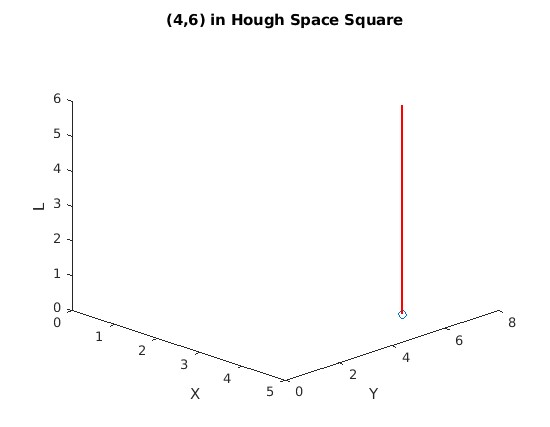
\includegraphics[width = 0.45\textwidth]{imgs/prob3_b.jpg}
    \caption{(4,6) square in Hough Square Space}
    \label{fig:prob3_b}
\end{figure}

\subsection*{C}

Here we are looking to describe all possible squares if we extend the previous example and discover an edge at $(6,8)$

\begin{figure}[H]
    \centering
    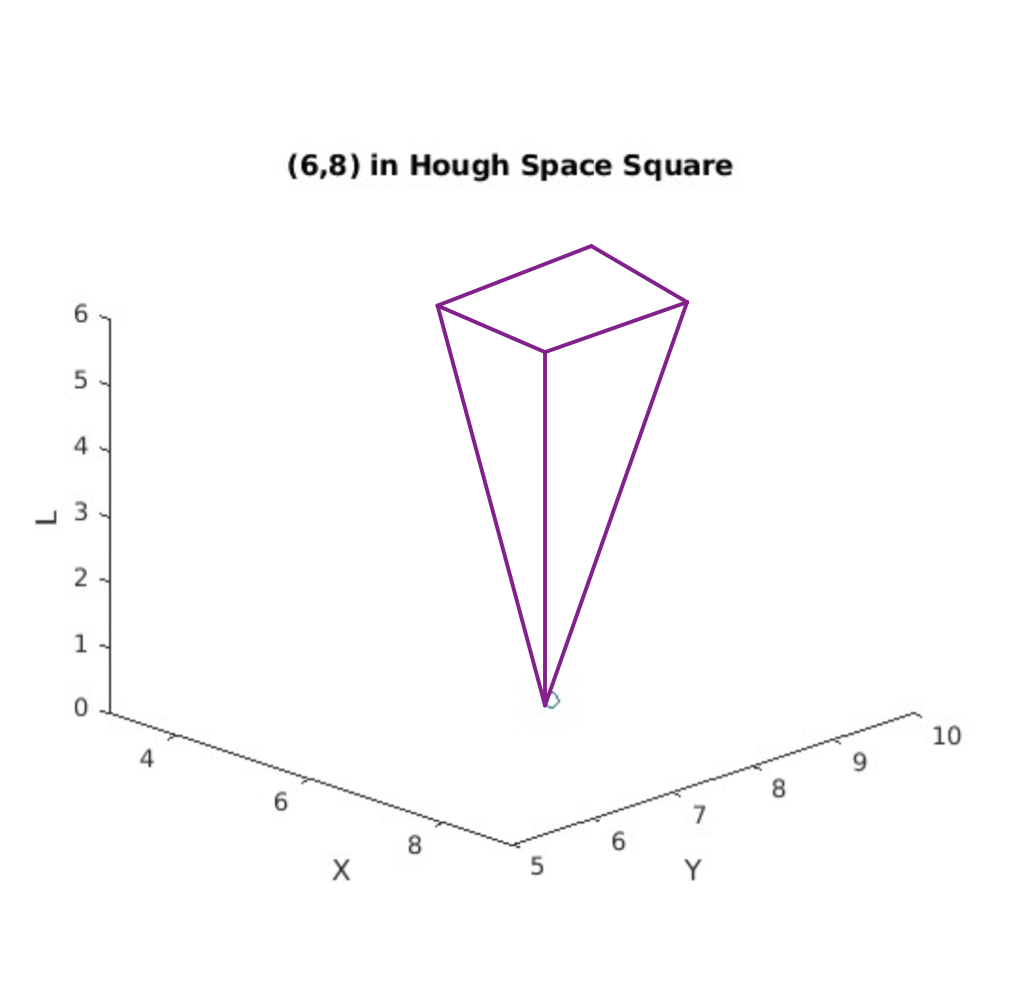
\includegraphics[width = 0.45\textwidth]{imgs/prob3_c.jpg}
    \caption{(6,8) square in Hough Square Space}
    \label{fig:prob3_c}
\end{figure}

Here we see a cone emenating from the $(6,8)$ point - as the size of the square increases, we radiate outwards in the possible length size $l$. This results in a pyramid (each layer being a square of the increased possible size. The center origin of the square is within the pyramid, and based on its position we know the resulting $l$ square side length.

\section*{Problem 4}

In this problem we are tasked with answering questions about Feature Detectors.

\subsection*{A}

In the SIFT detector, the local histogram of edge directions is computed; we are asked to explain briefly how this information is used and why it is needed. My response:

The edge directions allow us to identify and track the features (and thus objects) within a given image while being agnostic to a given image's lighting and, combined with other techniques, can even provide orientation agnostic labels to identify with.

\subsection*{B}

We are asked why in the HoG feature detector the $128x64$ window (height, width) is utiized. This is because the original HoG was focused on detecting humans - this window was discovered to be the most likely to properly frame humans in their dataset (twice as tall as wide) and thus used.

\end{document}